\section{Computational model}

        Il modello migliore è stato ottenuto dopo una prima fase di \textit{data preparation}, ed una successiva fase di \textit{hyper-parameter tuning}.

        \subsection{Data preparation}
        
                \subsubsection{Data splitting}
                
                        Il \textit{dataset} è stato diviso in due sezioni differenti:
                        \begin{itemize}
                                \item \textit{training set}: contiene 80\% dell'intero dataset originale (6400 records)
                                \item \textit{test set}: contiene il restante 20\% del dataset originale (1600 records)
                        \end{itemize}
                
                \subsubsection{Bad values management}
                
                        Il \textit{dataset} originale (\textit{training\_set.csv}) contiene dati mancanti in corrispondenza di alcune delle \textit{features}, per questo motivo, i valori relativi a tali campi sono stati sostituiti con la mediana relativa alla colonna della \textit{feature} corrispondente all'interno del \textit{dataset}.
                        \bigbreak
                        
                        In seguito, sono stati analizzati gli \textit{outliers}. Un \textit{outlier} è un'osservazione che devia marcatamente da altre osservazioni nel campione di dati. L'identificazione di potenziali \textit{outliers} è importante dal momento che potrebbero indicare dati corrotti o mal codificati, anche se, in alcuni casi, potrebbero essere il risultato di variazioni casuali nel campione di dati.
                        
                        L'individuazione degli \textit{outliers} dipende dalla distribuzione dei dati sottostante. Il \textit{dataset} considerato, come si evince dal pair-plot in figura \ref{fig:training_set_pairplot}, segua approssimativamente una distribuzione \textit{Normale}, pertanto sono stati analizzati i risultati derivanti da tre metodi:
                        \begin{itemize}
                            \item \textit{z-score}
                            \item \textit{modified z-score}
                            \item \textit{inter-quartile range}
                        \end{itemize}
                    
                        Lo \textit{Z-score} di una osservazione è definito come:
                        \begin{displaymath}
                                z_i = \frac{x_i - \mu_x}{\sigma}
                        \end{displaymath}
                        essendo $\mu_x$ e $\sigma$, rispettivamente, la media e la deviazione standard del campione di dati. Sono considerati \textit{outliers} i campioni con uno score maggiore di $3$.
                        \smallbreak
                        
                        Lo \textit{Z-score modificato} (\textit{Iglewicz and Hoaglin}) è definito come:
                        \begin{displaymath}
                                m_i = \frac{0.6745 \cdot (x_i - \tilde{x})}{MAD}
                        \end{displaymath}
                        essendo $MAD$ la median absolute deviation e $\tilde{x}$ la mediana. Sono considerati \textit{outliers} i campioni con uno score maggiore di $3.5$.
                        \smallbreak
                        
                        L'\textit{inter-quartile range} è definito come:
                        \begin{displaymath}
                                IQR = Q_3 - Q_1
                        \end{displaymath}
                        essendo $Q_1$ e $Q_3$, rispettivamente, il primo ed il terzo quartile del campione di dati. Sono considerati \textit{outliers} i campioni con uno valore maggiore di $Q_3 + IQR \cdot 1.5$ e minore di $Q_1 - IQR \cdot 1.5$.
                        \smallbreak
                        
                        Per non ridurre la numerosità del \textit{training set} si è scelto di sostituire (e non eliminare) gli \textit{outliers} con la mediana relativa ad una determinata \textit{feature}. Si è ritenuto opportuno utilizzare la mediana in quanto è una misura più robusta per la rappresentazione della dispersione di valori rispetto alla media essendo meno soggetta alla presenza di \textit{outliers}.                        
                
                \subsubsection{Data normalization}
                
                        \textbf{TODO}
                
                \subsubsection{Feature selection}
                
                        In questa fase sono state selezionate le \textit{features} più significative al fine di ridurre i costi di training e migliorare la capacità di generalizzazione del classificatore.
                        
                        \textbf{TODO}
                        
                        \begin{figure}[!h]
                            \centering
                            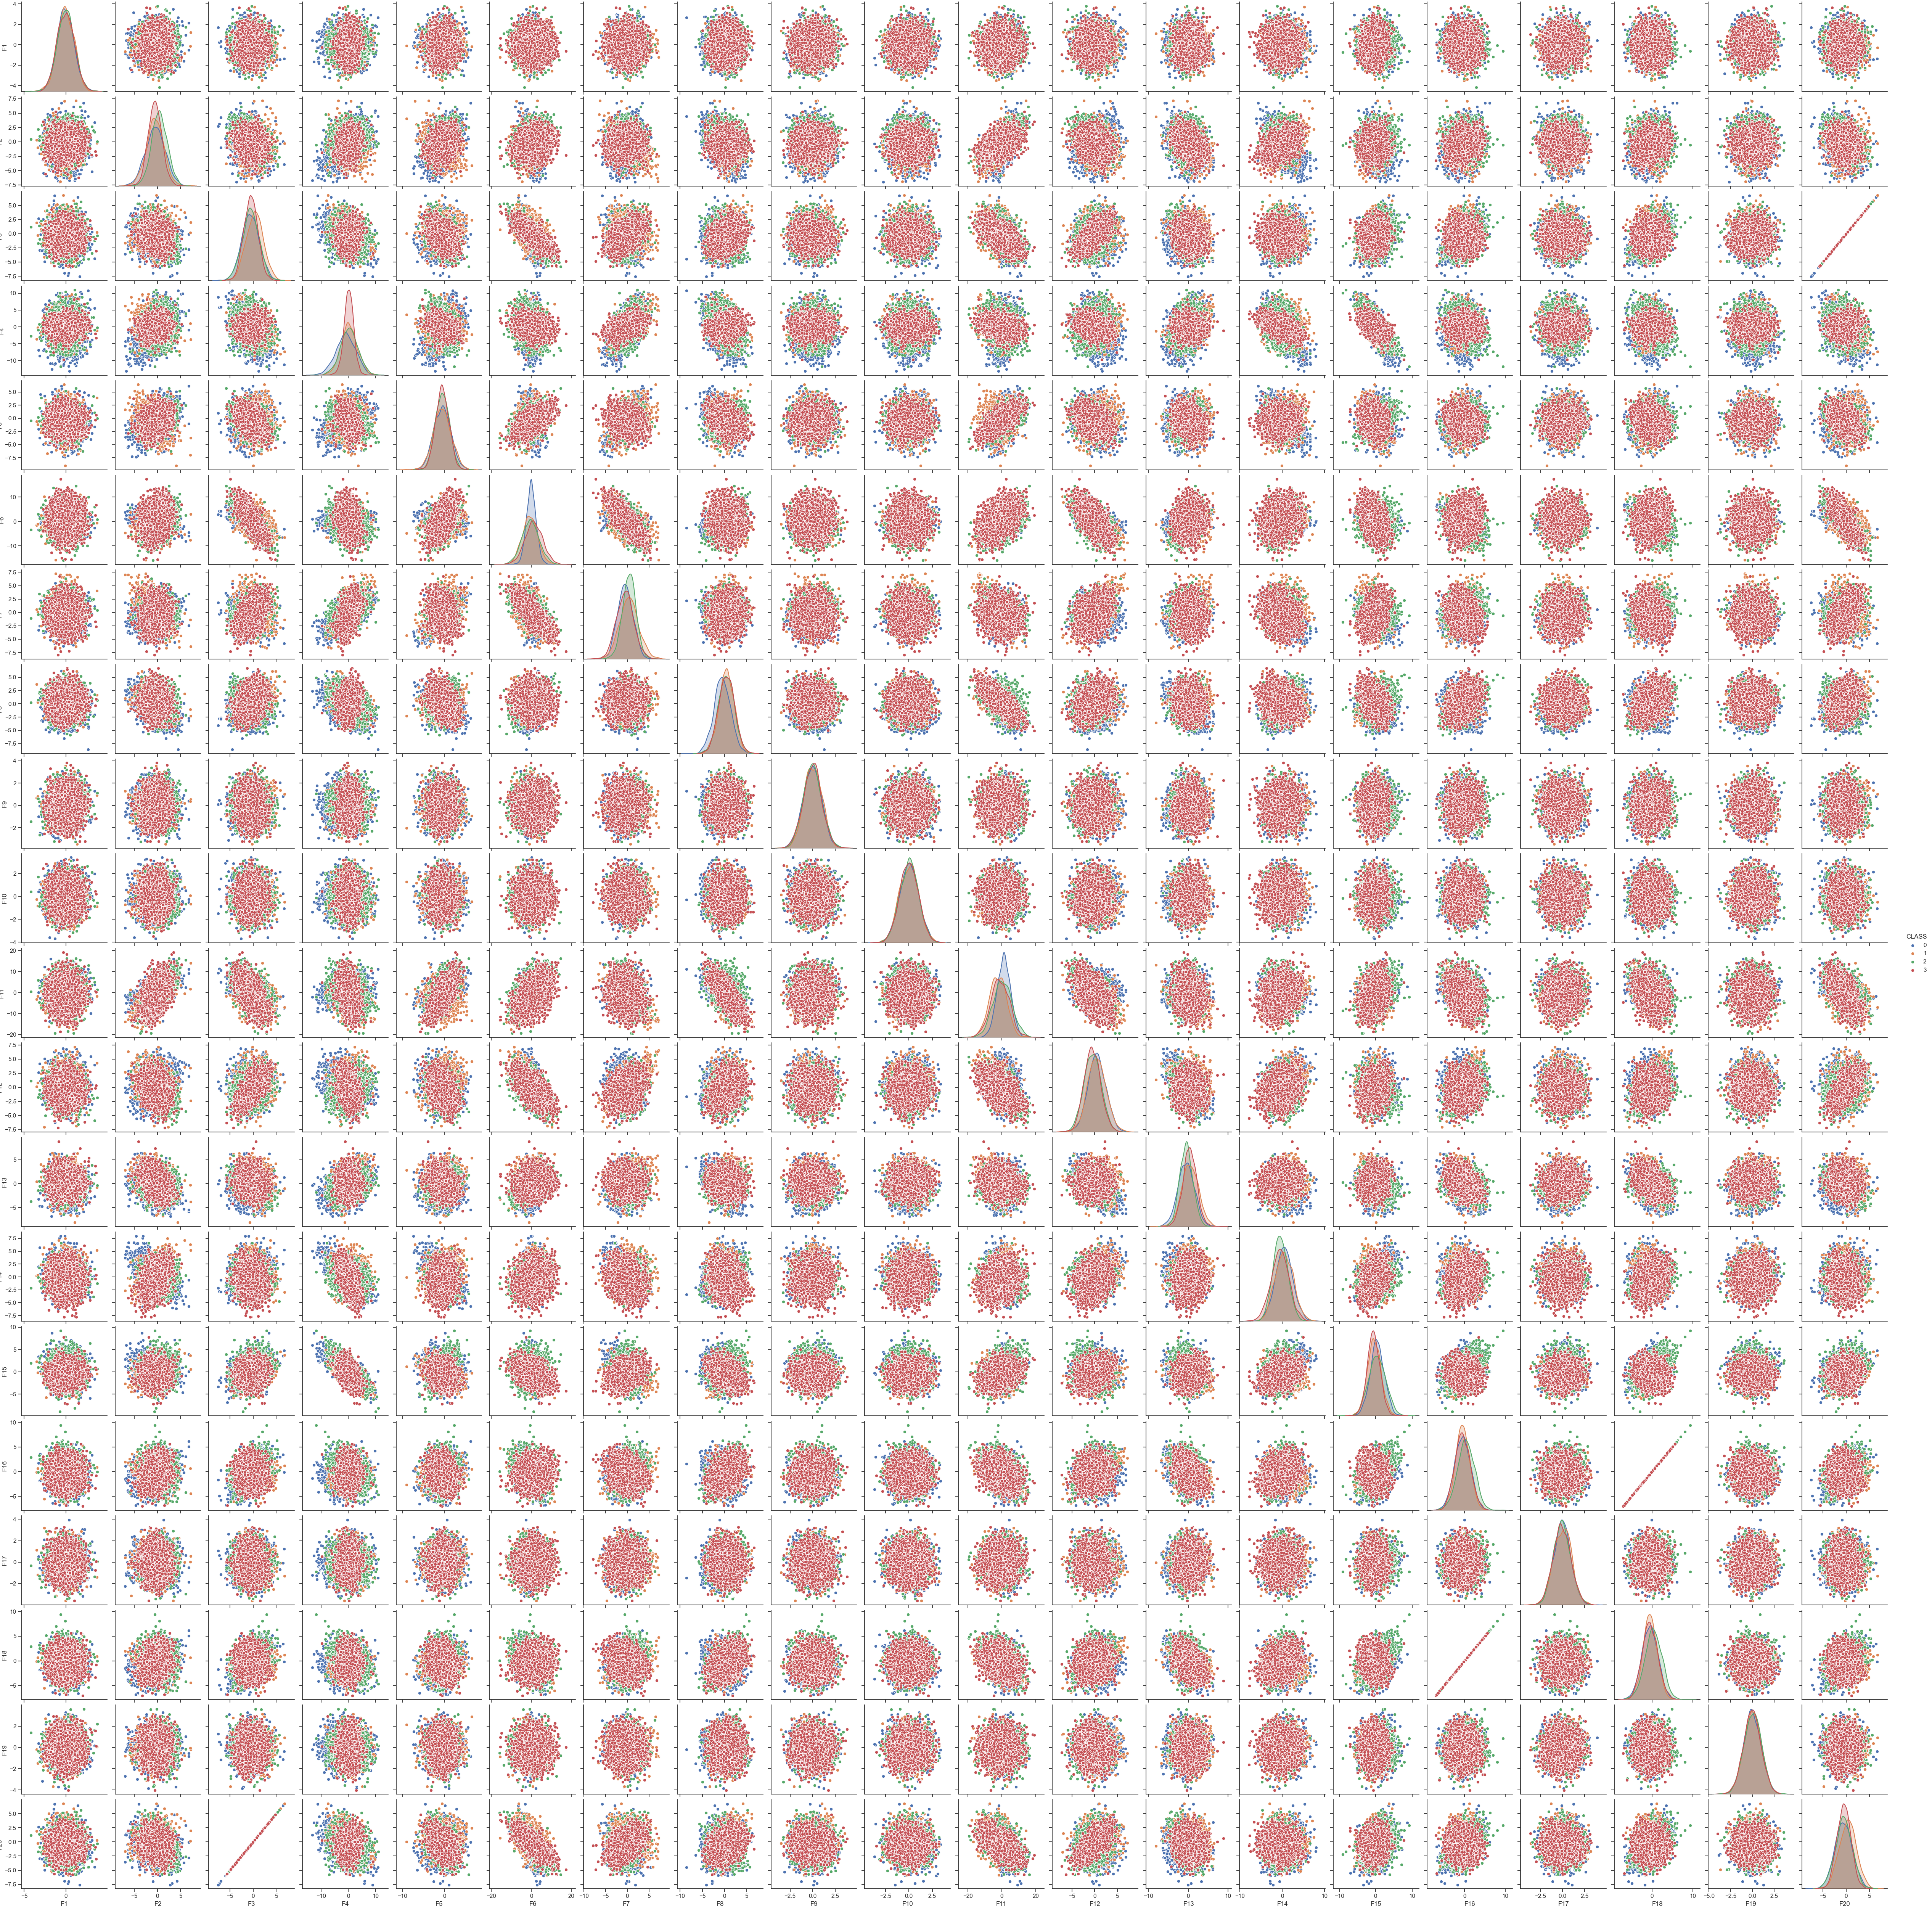
\includegraphics[width=175mm]{training_set}
                            \caption{Pair plot representing \textit{features}.}
                            \label{fig:training_set_pairplot}
                        \end{figure}
                        \clearpage
                
                \subsubsection{Data sampling} 
                
                        Il \textit{dataset} considerato presenta elementi così distribuiti:
                        \begin{itemize}
                                \item \textit{Class 1}: $33.67 \, \%$
                                \item \textit{Class 2}: $15.99 \, \%$
                                \item \textit{Class 3}: $20.66 \, \%$
                                \item \textit{Class 4}: $29.68 \, \%$
                        \end{itemize}
                        
                        \`E stato quindi effettuato balancing delle classi per evitare che il modello finale pecchi nel riconoscimento di classi meno presenti nel \textit{training set}.
                        
                        La tecnica di balancing utilizzata è lo \textit{SMOTE}.
                        
                        \textbf{TODO}
                

        \subsection{Hyper-parameters tuning}
        
                I modelli utilizzati per la classificazione sono:
                \begin{itemize}
                        \item \textit{Multi-Layer Perceptron}
                        \item \textit{Support Vector Machine}
                        \item \textit{Decition Tree}
                        \item \textit{Random Forest}
                        \item \textit{K-Nearest Neighbors}
                        \item \textit{Stochastic Gradient Descent}
                        \item \textit{Ada Boost}
                        \item \textit{Naive Bayes}
                        \item \textit{K-Means}
                \end{itemize}
            
                In questa fase sono stati cercati gli \textit{iper-parametri} per i vari classificatori.
                
                \textbf{TODO}
                

        \subsection{Evaluation}
        
                La metrica utilizzata al fine della valutazione dei classificatori è la \textit{f1-score} (media armonica), definita come segue:
                \begin{displaymath}
                F1 = \frac{2 \cdot precision \cdot recall}{precision + recall}
                \end{displaymath}
                con,
                \begin{displaymath}
                precision = \frac{TP}{TP + FP} \qquad recall = \frac{TP}{TP + FN}
                \end{displaymath}
                essendo $TN$ il numero di veri negativi, $FP$ il numero di falsi positivi, $FN$, falsi negativi e $TP$ veri positivi.